\chapter{矩阵与线性映射}
\label{chap:matrix}

上一章讨论了线性空间、线性空间同构以及基与坐标。选定基后，每个向量都可以由有限个坐标唯一表示；进一步地，线性空间同构对所有向量的作用，也可以由它对一组基中各个向量的作用完全确定。本章将从这些向量的坐标出发引出矩阵，再把线性空间同构推广为一般的线性映射，并研究线性映射的矩阵表示。

\section{矩阵的概念与运算}
\label{sec:matrix_origin}

在上一章中，我们介绍了线性空间同构的概念，但没有给出它的具体表示。对于域 \(\mathbb F\) 上的两个 \(n\) 维线性空间 \(V,W\)，给定一个线性空间同构
\[
    \varphi:V\to W.
\]
一个自然的问题是：映射 \(\varphi\) 的具体表达式是什么？为了清晰地描述这一映射，我们首先分别确定 \(V\) 和 \(W\) 的一组基：
\[
    \mathcal A=(\bm a_1,\ldots,\bm a_n),
    \quad
    \mathcal B=(\bm b_1,\ldots,\bm b_n).
\]
并且，对于\( V \)中的每个基向量 \(\bm a_j\)，都有 \(\varphi(\bm a_j)\in W\)与之对应。又由于 \(\mathcal B\) 是 \(W\) 的一组基，根据基表示的唯一性（\cref{thm:basis_unique}），存在唯一的一组标量 \(t_{1j},\ldots,t_{nj}\)，使得
\[
    \varphi(\bm a_j) = \sum_{i=1}^{n} t_{ij}\bm b_i.
\]
考虑\( V \)中的所有\( n \)个基向量，以及其在 \(W\) 中的像 \(\varphi(\bm a_j)\)的坐标表示，就可以得到 \(n^2\) 个系数 \(t_{ij}\)，其中\( i,j=1,\ldots,n \)。

接下来，任取 \(\bm v\in V\)，并设它在基 \(\mathcal A\) 下的坐标为 \((\alpha_1, \ldots, \alpha_n)\)，即
\[
    \bm v = \sum_{i=1}^{n} \alpha_i\bm a_i.
\]
由于线性空间同构保持向量加法和数乘，有
\[
    \begin{aligned}
        \varphi(\bm v)
         & = \varphi\left(\sum_{i=1}^{n} \alpha_i\bm a_i\right)=\sum_{j=1}^{n} \alpha_j \varphi(\bm a_j) = \sum_{j=1}^{n} \alpha_j \left( \sum_{i=1}^{n} t_{ij}\bm b_i \right) = \sum_{i=1}^{n} \left( \sum_{j=1}^{n} t_{ij}\alpha_j \right) \bm b_i.
    \end{aligned}
\]
因此，\(\varphi(\bm v)\) 在基 \(\mathcal B\) 下的第 \(i\) 个坐标\( \beta_i \)为
\[
    \beta_i = \sum_{j=1}^{n}t_{ij}\alpha_j.
\]
这意味着，只要知道前面得到的 \(n^2\) 个系数，对于任意向量 \(\bm v\in V\)，就可以通过上述公式计算出 \(\varphi(\bm v)\) 在基 \(\mathcal B\) 下的坐标。并且，对于这\( n^2 \)个系数，我们可以将其分为\( n \)组。自然，我们希望以二维的形式来记录这些系数，将\(\varphi(\bm a_j)\) 在基 \( \mathcal{B} \) 下的坐标排在第 \(j\) 列，得到
\[
    \mathbf{T}=
    \begin{bmatrix}
        t_{11} & t_{12} & \cdots & t_{1n} \\
        t_{21} & t_{22} & \cdots & t_{2n} \\
        \vdots & \vdots & \ddots & \vdots \\
        t_{n1} & t_{n2} & \cdots & t_{nn}
    \end{bmatrix}.
\]
这个二维数组完整记录了同构 \(\varphi\) 在所选基下的作用。

\begin{example}
    \label{ex:linear_map_matrix}
    如\cref{fig_linear_map_square_shear} 所示，有一线性同构\(\varphi\) 可以将 \(V\) 中的单位正方形映成 \(W\) 中的一个平行四边形。

    \begin{center}
        \captionsetup{type=figure}
        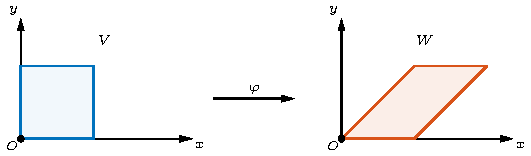
\includegraphics{./img/2-matrix/linear_map_square_shear.pdf}
        \captionof{figure}{矩阵 \(\mathbf T\) 所表示的线性空间同构对单位正方形的作用}
        \label{fig_linear_map_square_shear}
    \end{center}

    对于映射前后的两个线性空间 \(V=W=\mathbb R^2\)，不妨都选取标准基
    \[
        \mathcal A=\mathcal B=\left(\bm e_1,\bm e_2\right).
    \]

    那么，对于 \(V\) 中的任意向量 \(\bm v\)，设它在基 \(\mathcal A\) 下的坐标为
    \((\alpha_1,\alpha_2)\)。通过观察图形，可以发现映射后的向量 \(\varphi(\bm v)\)，在
    \(\mathcal B\) 下的坐标为 \((\beta_1,\beta_2)\)，并且满足
    \[
        \begin{cases}
            \beta_1=\alpha_1+\alpha_2, \\
            \beta_2=\alpha_2,
        \end{cases}
    \]
    因此，这一同构可以用如下矩阵表示
    \[
        \mathbf T=
        \begin{bmatrix}
            1 & 1 \\
            0 & 1
        \end{bmatrix}.
    \]
    几何上，像这样的变换被称作剪切变换，对应的矩阵称为剪切矩阵。
\end{example}


注意到，上述推导中的线性空间 \(V\) 与 \(W\) 维数相同，因此得到的是一个方形数组。但上述推导实际只使用了映射保持向量加法和数乘，并没有使用它是双射这一条件。因此，可以令定义域的维数为 \(n\)，陪域的维数为 \(m\)，推导过程同样成立。最终得到 \(mn\) 个系数，并将它们排列为 \(m\) 行 \(n\) 列。基于这一观察，可以给出一般矩阵的定义。

\begin{definition}[矩阵]
    \label{def:matrix}
    设 \(m,n\) 是非负整数，\(\mathbb F\) 是一个域。由 \(mn\) 个属于 \(\mathbb F\) 的元素按照 \(m\) 行 \(n\) 列排列成的矩形数组
    \[
        \mathbf{A}=
        \begin{bmatrix}
            a_{11} & a_{12} & \cdots & a_{1n} \\
            a_{21} & a_{22} & \cdots & a_{2n} \\
            \vdots & \vdots & \ddots & \vdots \\
            a_{m1} & a_{m2} & \cdots & a_{mn}
        \end{bmatrix} = [a_{ij}]_{m \times n}
    \]
    称为一个 \(m\times n\) \textbf{矩阵}（Matrix），通常使用加粗正体字母表示\footnote{如果矩阵大小已知，那么\( [a_{ij}]_{m \times n} \)可以简记为\( [a_{ij}] \)。}。其中，\(a_{ij}\) 称为矩阵 \(\mathbf{A}\) 的第 \(i\) 行第 \(j\) 列元素。所有 \(\mathbb F\) 上的 \(m\times n\) 矩阵组成的集合记作 \(\mathbb{F}^{m \times n}\)。
\end{definition}

有了矩阵之后，标量乃至向量都可以表示为一个矩阵。比如一个标量可以看作是一个\( 1 \times 1 \)的矩阵，而向量即可以看作是一个 \(n \times 1\) 的列矩阵（列向量）\footnote{在本书中，除非特别说明，向量默认表示为列向量。}，也可以看作是一个 \(1 \times n\) 的行矩阵（行向量）。

进一步地，向量组同样可以使用矩阵表示。按照列向量的默认约定，对于一个\( m \times n \)的矩阵，其可以看作是 \(n\) 个 \(m\) 维列向量组成的向量组。因此，向量组的一些概念，比如张成、秩等，都可以直接用矩阵来表示。比如，\( \operatorname{span}(\mathbf{T}) \)和\( \operatorname{rank}(\mathbf{T}) \)分别表示由矩阵 \(\mathbf{T}\) 的列向量构成的向量组的张成和秩。

类似于向量，两个矩阵相等，当且仅当它们的行数和列数分别相同，并且对应位置的元素都相等。所有元素均为 \(0\) 的 \(m\times n\) 矩阵称为\textbf{零矩阵}，记作 \(\mathbf{0}\)。并且，矩阵的加法和数乘都按照对应位置的元素进行。

\begin{definition}[矩阵加法与数乘]
    \label{def:matrix_add_scalar}
    设 \(\mathbf{A}=(a_{ij}),\mathbf{B}=(b_{ij})\in \mathbb{F}^{m \times n}\)，\(\lambda\in\mathbb F\)，定义
    \[
        \mathbf{A}+\mathbf{B}=(a_{ij}+b_{ij}),
        \quad
        \lambda \mathbf{A}=(\lambda a_{ij}).
    \]
\end{definition}

由域中加法和乘法的运算律可以直接验证：\(\mathbb{F}^{m \times n}\) 在上述运算下构成 \(\mathbb F\) 上的线性空间。既然\( \mathbb{F}^{m \times n} \)是一个线性空间，自然也可以选取一组基。最简单的一组基由\( \mathbf{E}_{ij} \)这样的矩阵组成，其中第 \(i\) 行第 \(j\) 列元素为 \(1\)，其余元素均为 \(0\)。在这组基下，任意矩阵 \(\mathbf{A}=(a_{ij})\) 都可以唯一写成
\[
    \mathbf{A}=\sum_{i=1}^{m}\sum_{j=1}^{n}a_{ij}\mathbf{E}_{ij}.
\]
因此，该线性空间的维数为 \(mn\)，即
\[
    \dim \mathbb{F}^{m \times n}=mn.
\]

转置同样是矩阵的一个基本运算。它将矩阵的行与列互换，得到一个新的矩阵。

\begin{definition}[转置]
    \label{def:matrix_transpose}
    设 \(\mathbf{A}=(a_{ij})\in \mathbb{F}^{m \times n}\)。由
    \[
        (\mathbf{A}^{\mathsf T})_{ij}=a_{ji}
    \]
    定义的 \(n\times m\) 矩阵 \(\mathbf{A}^{\mathsf T}\) 称为 \(\mathbf{A}\) 的\textbf{转置矩阵}（Transpose）。
\end{definition}

例如，下方的\( 2 \times 3 \)的矩阵的转置为一个 \(3 \times 2\) 的矩阵：
\[
    \begin{bmatrix}
        1 & 2 & 3 \\
        4 & 5 & 6
    \end{bmatrix}^{\mathsf T}
    =
    \begin{bmatrix}
        1 & 4 \\
        2 & 5 \\
        3 & 6
    \end{bmatrix}.
\]
此外，根据定义可以验证
\[
    (\mathbf{A}+\mathbf{B})^{\mathsf T}=\mathbf{A}^{\mathsf T}+\mathbf{B}^{\mathsf T},
    \quad
    (\lambda \mathbf{A})^{\mathsf T}=\lambda \mathbf{A}^{\mathsf T},
    \quad
    (\mathbf{A}^{\mathsf T})^{\mathsf T}=\mathbf{A}.
\]

对于转置后的矩阵，\( \operatorname{span}(\mathbf{A}^{\mathsf{T}}) \)和\( \operatorname{rank}(\mathbf{A}^{\mathsf{T}}) \)分别表示由矩阵 \(\mathbf{A}\) 的行向量构成的向量组的张成和秩。尽管其几何意义与\( \operatorname{span}(\mathbf{A}) \)和\( \operatorname{rank}(\mathbf{A}) \)完全不同，但结果却不一定不同。事实上，矩阵的行秩与列秩总是相等的，即
\[
    \operatorname{rank}(\mathbf{A})=\operatorname{rank}(\mathbf{A}^{\mathsf{T}}).
\]
在后面的章节中，我们将给出对应的证明。

\section{线性映射与矩阵乘法}
\label{sec:linear_map}

在上一章中，我们通过推导发现，一个线性空间同构可以由一个方阵来表示。并指出，如果定义域与陪域的维数不同，可以得到一个更一般的矩阵。对于这个更一般的矩阵，其对应的映射不再是同构，而是一个更一般的映射，称为线性映射。

\begin{definition}[线性映射]
    \label{def:linear_map}
    设 \(V,W\) 是域 \(\mathbb F\) 上的两个线性空间。映射 \(T:V\to W\) 如果对于任意 \(\bm u,\bm v\in V\) 和任意 \(\lambda\in\mathbb F\)，都有
    \[
        T(\bm u+\bm v)=T(\bm u)+T(\bm v),
        \quad
        T(\lambda\bm v)=\lambda T(\bm v),
    \]
    则称 \(T\) 是从 \(V\) 到 \(W\) 的一个\textbf{线性映射}（Linear Map）。如果 \(V=W\)，则称 \(T\) 是 \(V\) 上的一个\textbf{线性变换}（Linear Transformation）。
\end{definition}

需要注意的是，线性变换并不一定是线性空间同构的。例如，\textbf{零映射} \(T:V\to V\) 定义为 \(T(\bm v)=\bm 0\) 对任意 \(\bm v\in V\) 成立。显然，它将\( V \)中的向量仍然映射到 \( V \) 中，但它不是双射，因此不是同构。此外，还有一种特殊的线性映射，其将每个向量映射到它自身，这种映射称为\textbf{恒等映射}，通常记作\(I\)。

从\cref{def:linear_map}可以看出，线性映射要求保持向量加法和数乘。换句话说，线性映射是保持线性结构的映射。如\cref{fig:linear_map}所示，其背后的几何意义非常明确。

\begin{figure}[htb!]
    \centering
    \begin{subfigure}{0.75\textwidth}
        \centering
        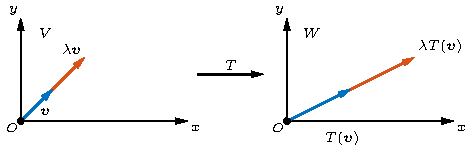
\includegraphics{./img/2-matrix/linear_map_scalar_mult.pdf}
        \caption{数乘不变}
        \label{fig:linear_map_scalar_mult}
    \end{subfigure}
    \begin{subfigure}{0.75\textwidth}
        \centering
        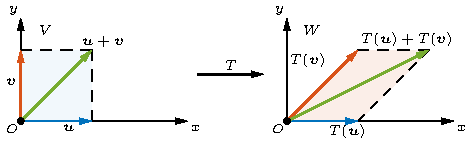
\includegraphics{./img/2-matrix/linear_map_addition.pdf}
        \caption{向量加法不变}
        \label{fig:linear_map_addition}
    \end{subfigure}
    \caption{线性映射保持线性结构}
    \label{fig:linear_map}
\end{figure}

而如下的例子，则进一步展示出线性映射不仅仅局限于几何图像，还可以应用于更一般的线性空间。
\begin{example}
    \label{ex:derivative_linear_map}
    对于正整数 \(n\)，定义求导映射
    \[
        D:\mathcal P_n\to\mathcal P_{n-1}, \quad D(p)=p',
    \]
    其中 \(p\in\mathcal P_n\)为次数不超过 \(n\) 的实系数多项式， \(p'\) 为其导数。容易验证，对于任意 \(p,q\in\mathcal P_n\) 和 \(\lambda\in\mathbb R\)，有
    \[
        D(p+q)=p'+q'=D(p)+D(q),
        \quad
        D(\lambda p)=\lambda p'=\lambda D(p),
    \]
    因此求导映射 \(D\) 是线性映射。
\end{example}

正如上一章所述，对于线性变换\( T: V \to W  \)，在选定基后，可以用一个矩阵\( \mathbf{T} = [t_{ij}] \)来表示。下方的定义则给出了更严谨的表述。

\begin{definition}[线性映射的表示矩阵]
    \label{def:representation_matrix}
    设 \(V\) 和\(W\) 是域 \(\mathbb F\) 上的线性空间，而\( \mathcal A=(\bm a_1,\ldots,\bm a_n) \)和\( \mathcal B=(\bm b_1,\ldots,\bm b_m) \)分别是两个线性空间上的一组基。若\(T:V\to W\) 是线性映射，并且\( V \)中的每个基向量 \(\bm a_j\) 在 \(W\) 中的像 \(T(\bm a_j)\) 在基 \(\mathcal B\) 下的坐标为
    \[
        T(\bm a_j) = \sum_{i=1}^{m} t_{ij}\bm b_i, \quad j=1,\ldots,n,
    \]
    则称矩阵
    \[
        \mathbf{T}=
        \begin{bmatrix}
            t_{11} & t_{12} & \cdots & t_{1n} \\
            t_{21} & t_{22} & \cdots & t_{2n} \\
            \vdots & \vdots & \ddots & \vdots \\
            t_{m1} & t_{m2} & \cdots & t_{mn}
        \end{bmatrix}
    \]
    为线性映射 \(T\) 在基 \(\mathcal A\) 和 \(\mathcal B\) 下的\textbf{表示矩阵}（Representation Matrix）。
\end{definition}

将所有从 \(V\) 到 \(W\) 的线性映射组成的集合记作 \(\mathcal L(V,W)\)，并且对于任意 \(S,T\in\mathcal L(V,W)\)、\(\lambda\in\mathbb F\) 和 \(\bm v\in V\)，定义如下映射上的加法和数乘：
\[
    (S+T)(\bm v)=S(\bm v)+T(\bm v),
    \quad
    (\lambda T)(\bm v)=\lambda T(\bm v).
\]
可以验证，\(\mathcal L(V,W)\) 在上述运算下构成 \(\mathbb F\) 上的线性空间。固定 \(V\) 和 \(W\) 的基后，这一线性空间与相应的矩阵空间同构。

\begin{theorem}[线性映射空间与矩阵空间的同构]
    \label{thm:linear_map_matrix_space_isomorphism}
    设 \(V,W\) 是域 \(\mathbb F\) 上的有限维线性空间，\(\dim V=n\)，\(\dim W=m\)，并分别固定 \(V\) 和 \(W\) 的基 \(\mathcal A\) 和 \(\mathcal B\)。则
    \[
        \mathcal L(V,W)\cong\mathbb F^{m\times n}.
    \]
\end{theorem}

\begin{proof}
    将每个线性映射 \(T\in\mathcal L(V,W)\) 对应到它在基 \(\mathcal A\) 和 \(\mathcal B\) 下的表示矩阵 \(\mathbf T\)，记这一对应为
    \[
        \Phi:\mathcal L(V,W)\to\mathbb F^{m\times n},
        \quad
        \Phi(T)=\mathbf T.
    \]
    先证明 \(\Phi\) 保持加法和数乘。设 \(S,T\in\mathcal L(V,W)\) 的表示矩阵分别为 \(\mathbf S=[s_{ij}]\) 和 \(\mathbf T=[t_{ij}]\)，并取 \(\lambda\in\mathbb F\)。对于基 \(\mathcal A\) 中的每个基向量 \(\bm a_j\)，有
    \[
        (S+T)(\bm a_j)
        =\sum_{i=1}^{m}(s_{ij}+t_{ij})\bm b_i,
    \]
    因此 \(S+T\) 的表示矩阵为 \(\mathbf S+\mathbf T\)。类似地，\(\lambda T\) 的表示矩阵为 \(\lambda\mathbf T\)，所以
    \[
        \Phi(S+T)=\Phi(S)+\Phi(T),
        \quad
        \Phi(\lambda T)=\lambda\Phi(T).
    \]
    这说明 \(\Phi\) 是线性映射。

    由 \cref{def:representation_matrix} 可知，对于每一个线性映射 \(T\in\mathcal L(V,W)\)，都有唯一的表示矩阵 \(\mathbf T\) 与之对应，因此 \(\Phi\) 是双射。综上，\(\Phi\) 是线性空间同构，故
    \[
        \mathcal L(V,W)\cong\mathbb F^{m\times n}.
    \]
\end{proof}

如前一节所述，设\( V \)的任意一个向量\( \bm{v} \)，以及其在\( W \)中的像\( T(\bm{v}) \)，在对应的基下的坐标表示为
\[
    \bm{\alpha} = \begin{bmatrix} \alpha_1 &  \cdots & \alpha_n \end{bmatrix}^{\mathsf{T}} \in \mathbb{R}^n, \quad
    \bm{\beta} = \begin{bmatrix} \beta_1 &  \cdots & \beta_m \end{bmatrix}^{\mathsf{T}} \in \mathbb{R}^m.
\]
那么，这两个坐标之间满足如下关系：
\[
    \beta_i = \sum_{j=1}^{n} t_{ij} \alpha_j, \quad i = 1, \ldots, m.
\]
显然，在上式中，矩阵\( \mathbf{T} \)与向量\( \bm{\alpha} \)进行运算，得到了一个新的向量\( \bm{\beta} \)。由此可以定义矩阵与向量的乘法，如下所示。
\begin{definition}[矩阵与向量的乘法]
    \label{def:matrix_vector_mult}
    设 \(\mathbf{A}=[a_{ij}]\in \mathbb{F}^{m \times n}\)，\(\bm x=[x_1,\ldots,x_n]^{\mathsf T}\in \mathbb{F}^n\)。定义矩阵 \(\mathbf{A}\) 与向量 \(\bm x\) 的乘积为
    \[
        \bm{y} = \mathbf{A}\bm x \in \mathbb{F}^m,
    \]
    其中向量\( \bm{y} \)的第\( i \)个元素为\(y_i=\sum_{j=1}^{n}a_{ij}x_j\)。
\end{definition}

例如，设
\[
    \mathbf{A}=
    \begin{bmatrix}
        1 & 2 & 3 \\
        4 & 5 & 6
    \end{bmatrix},
    \quad
    \bm x=
    \begin{bmatrix}
        1 \\
        2 \\
        3
    \end{bmatrix},
\]
则
\[
    \mathbf{A}\bm x=
    \begin{bmatrix}
        1\times 1 + 2\times 2 + 3\times 3 \\
        4\times 1 + 5\times 2 + 6\times 3
    \end{bmatrix}=
    \begin{bmatrix}14 \\
        32
    \end{bmatrix}.
\]

\cref{fig_linear_map_square_shear}展示的仿射变换，在两个线性空间均选取标准基的情况下，可以用矩阵表示为
\[
    \mathbf{T}=
    \begin{bmatrix}
        1 & 1 \\
        0 & 1
    \end{bmatrix}.
\]
因此，对于\( V \)中的坐标向量\( [\alpha_1, \alpha_2]^{\mathsf{T}} \)，有映射后的坐标向量为
\[
    \begin{bmatrix}
        \beta_1 \\
        \beta_2
    \end{bmatrix}=
    \begin{bmatrix}
        1 & 1 \\
        0 & 1
    \end{bmatrix}
    \begin{bmatrix}
        \alpha_1 \\
        \alpha_2
    \end{bmatrix}=
    \begin{bmatrix}
        \alpha_1 + \alpha_2 \\
        \alpha_2
    \end{bmatrix}.
\]
这一代数运算结果与几何图形的变换完全一致。

与此同时，在两个\(\mathbb{R}^n\)线性空间均选取标准基的情况下，零映射和恒等映射分别可以用如下矩阵表示：
\[
    \mathbf{0}=
    \begin{bmatrix}
        0      & 0      & \cdots & 0      \\
        0      & 0      & \cdots & 0      \\
        \vdots & \vdots & \ddots & \vdots \\
        0      & 0      & \cdots & 0
    \end{bmatrix},
    \quad
    \mathbf{I}=
    \begin{bmatrix}
        1      & 0      & \cdots & 0      \\
        0      & 1      & \cdots & 0      \\
        \vdots & \vdots & \ddots & \vdots \\
        0      & 0      & \cdots & 1
    \end{bmatrix}.
\]
像这样全部由 \(0\)组成的矩阵（不一定是方阵）称为\textbf{零矩阵}，而对角线上全部为 \(1\) 且其余元素均为 \(0\) 的方阵称为\textbf{单位矩阵}。

有意思的是，仔细观察\cref{def:matrix_vector_mult}，可以发现矩阵与向量的乘法非常适合用于表示向量组的线性组合。设矩阵 \(\mathbf{A}=[\bm a_1,\ldots,\bm a_n]\in \mathbb{F}^{m \times n}\)，其中每一列向量\(\bm a_j\in \mathbb{F}^m\)。那么，对于任意向量\(\bm x=[x_1,\ldots,x_n]^{\mathsf T}\in \mathbb{F}^n\)，有
\[
    \mathbf{A}\bm x = \begin{bmatrix}
        \bm a_1 & \ldots & \bm a_n
    \end{bmatrix} \begin{bmatrix}
        x_1    \\
        \vdots \\
        x_n
    \end{bmatrix}
    = x_1\bm a_1 + \ldots + x_n\bm a_n = \sum_{j=1}^{n}x_j\bm a_j.
\]
这一观察使得我们无需记忆\cref{def:matrix_vector_mult}中的复杂的求和公式，而只需记住矩阵与向量的乘法就是将矩阵的列向量按向量的坐标进行线性组合，即可计算出结果。

或者，我们也可以将矩阵\( \mathbf{A} \)拆分成多个行向量\footnote{这里的行向量\( \bm{a}_i^{\mathsf{T}} \)表示矩阵的第 \(i\) 行，和前面提到的列向量\( \bm{a}_j \)取值并不相同。}，即
\[
    \mathbf{A}=
    \begin{bmatrix}
        \bm a^{\mathsf T}_1 \\
        \vdots              \\
        \bm a^{\mathsf T}_m
    \end{bmatrix},
\]
此时，矩阵与向量的乘法可以写成
\[
    \mathbf{A}\bm x =
    \begin{bmatrix}
        \bm a^{\mathsf T}_1 \\
        \vdots              \\
        \bm a^{\mathsf T}_m\bm x
    \end{bmatrix} \bm{x} =
    \begin{bmatrix}
        \bm a^{\mathsf T}_1\bm x \\
        \vdots                   \\
        \bm a^{\mathsf T}_m\bm x
    \end{bmatrix}
\]
其中, \( \bm a^{\mathsf T}_i\bm x \)可以看作是一个\( 1 \times n \)的矩阵乘上一个\( n \times 1 \)的向量，结果是一个\( 1 \times 1 \)的矩阵，即一个标量。并且，矩阵的第 \(i\) 行与向量\( \bm{x} \)的乘积得到就是最终结果的第 \(i\) 个元素。

接下来，让我们考虑这样一个问题：设有线性映射 \(T:V\to W\)和线性映射 \(S:W\to U\)。它们的复合映射 \(S\circ T:V\to U\) 定义为
\[
    (S\circ T)(\bm v) = S(T(\bm v)), \quad \bm v\in V.
\]
显然，复合映射 \(S\circ T\) 仍然是线性映射。在一组固定的基下，\(T\) 和 \(S\) 分别有表示矩阵 \(\mathbf{T} \in \mathbb{F}^{m \times n}\) 和 \(\mathbf{S} \in \mathbb{F}^{p \times m}\)。那么，复合映射 \(S\circ T\) 的表示矩阵是什么呢？

设有\( V \)中的向量的坐标\( \bm{\alpha} \in \mathbb{F}^n \)，则该向量在 \(W\) 中的像的坐标为
\[
    \bm{\beta} = \mathbf{T}\bm{\alpha} \in \mathbb{F}^m.
\]
进一步地，该向量在 \(U\) 中的像的坐标为
\[
    \bm{\gamma} = \mathbf{S}\bm{\beta} = \mathbf{S}(\mathbf{T}\bm{\alpha}) \in \mathbb{F}^p.
\]
将上述运算写成元素的形式，有
\[
    \gamma_i = \sum_{k=1}^{m} s_{ik}\beta_k = \sum_{k=1}^{m} s_{ik}\left(\sum_{j=1}^{n} t_{kj}\alpha_j\right) = \sum_{j=1}^{n}\left(\sum_{k=1}^{m} s_{ik}t_{kj}\right)\alpha_j, \quad i = 1, \ldots, p.
\]

直觉上，我们希望定义某种矩阵与矩阵之间的乘法，使得
\[
    \mathbf{S}\mathbf{T} = \left[\sum_{k=1}^{m} s_{ik}t_{kj}\right]_{p \times n},
\]
如此一来，复合映射 \(S\circ T\) 的表示矩阵就是矩阵 \(\mathbf{S}\) 与 \(\mathbf{T}\) 的乘积 \(\mathbf{S}\mathbf{T}\)
\[
    \bm{\gamma} = \mathbf{S}(\mathbf{T} \bm{\alpha}) = (\mathbf{S}\mathbf{T})\bm{\alpha}.
\]
这一观察使得我们可以定义矩阵与矩阵之间的乘法，如下所示。
\begin{definition}[矩阵的乘法]
    \label{def:matrix_mult}
    设 \(\mathbf{A}=[a_{ij}]\in \mathbb{F}^{m \times p}\)，\(\mathbf{B}=[b_{ij}]\in \mathbb{F}^{p \times n}\)。定义矩阵 \(\mathbf{A}\) 与矩阵 \(\mathbf{B}\) 的乘积为
    \[
        \mathbf{C} = \mathbf{A}\mathbf{B} \in \mathbb{F}^{m \times n},
    \]
    其中矩阵 \( \mathbf{C} = [c_{ij}] \)的第\( i \)行第\( j \)列元素为
    \[
        c_{ij} = \sum_{k=1}^{p} a_{ik} b_{kj}.
    \]
\end{definition}

比如，设
\[
    \mathbf{A}=
    \begin{bmatrix}
        1 & 2 & 3 \\
        4 & 5 & 6
    \end{bmatrix},
    \quad
    \mathbf{B}=
    \begin{bmatrix}
        7  & 8  \\
        9  & 10 \\
        11 & 12
    \end{bmatrix},
\]
则
\[
    \mathbf{A}\mathbf{B}=
    \begin{bmatrix}
        1\times 7 + 2\times 9 + 3\times 11 & 1\times 8 + 2\times 10 + 3\times 12 \\
        4\times 7 + 5\times 9 + 6\times 11 & 4\times 8 + 5\times 10 + 6\times 12
    \end{bmatrix}=
    \begin{bmatrix}
        58  & 64  \\
        139 & 154
    \end{bmatrix}.
\]

可以通过将矩阵乘法拆分为多个矩阵与向量的乘法来进行运算，令矩阵\( \mathbf{B} = [\bm b_1, \ldots, \bm b_n] \)，则有
\[
    \mathbf{A}\mathbf{B} = \mathbf{A} \begin{bmatrix}
        \bm b_1 & \ldots & \bm b_n
    \end{bmatrix} =\begin{bmatrix}
        \mathbf{A}\bm b_1 & \ldots & \mathbf{A}\bm b_n
    \end{bmatrix}.
\]
进一步地，如果将矩阵\( \mathbf{A} \)拆分为多个行向量，即\( \mathbf{A} = [\bm{a}_1, \ldots, \bm{a}_m]^{\mathsf{T}} \)，则有
\[
    \mathbf{A}\mathbf{B} =
    \begin{bmatrix}
        \bm a^{\mathsf T}_1 \\
        \vdots              \\
        \bm a^{\mathsf T}_m
    \end{bmatrix}
    \begin{bmatrix}
        \bm b_1 & \ldots & \bm b_n
    \end{bmatrix} =
    \begin{bmatrix}
        \bm a^{\mathsf T}_1\bm b_1 & \ldots & \bm a^{\mathsf T}_1\bm b_n \\
        \vdots                     &        & \vdots                     \\
        \bm a^{\mathsf T}_m\bm b_1 & \ldots & \bm a^{\mathsf T}_m\bm b_n
    \end{bmatrix}.
\]
观察可以发现，矩阵\( \mathbf{A} \)和\( \mathbf{B} \)的乘积的第\( i \)行第\( j \)列元素就是矩阵\( \mathbf{A} \)的第\( i \)行与矩阵\( \mathbf{B} \)的第\( j \)列的乘积\( \bm{a}_i^{\mathsf{T}}\bm b_j \)。

\section{矩阵乘法的基本性质}
